
\documentclass[11pt]{article}

\marginparwidth 0.2in 
\oddsidemargin 0.1in 
\evensidemargin 0.1in 
\marginparsep 0.1in
\topmargin 0.1in 
\textwidth 6.5in \textheight 8 in

\usepackage[counterclockwise, figuresleft]{rotating}
\usepackage{hyperref}  
\usepackage{listings}
\usepackage{array}
\usepackage{tabularx}
\usepackage{attachfile}

\begin{document}

\author{İbrahim Burak Tanrıkulu, 21827852}
\title{BBM436 Microprocessors Lab.\\Assignment 5\\I/O Map}
\maketitle

\section{Basic one byte input/output}
In this part, i used two 4x4 keypads for input and 2 7-segment display to output. Also used IN and OUT instructions in my assembly code.\\
While taking an input, i put some delay for pressing buttons. When delay is finished, IN instruction gives an address and creates RD signal to read.\\
Input address is 00H. This address enables "Input Latch" and data comes to microprocessor from "Tranceiver".\\
Output address is 01H. This address disables "Input Latch". OUT instruction creates WR signal which is enables "Output Latch" and we can see our input at 7-segment displays.\\
You can find first part here: \attachfile{Project1.pdsprj}\\
You can see project image here: \ref{Tasarım}
\section{10 digit 7-segment display}
In this part I used two different outputs for displaying 10 digit integer. First is "Led Select". Used a "4 to 10 decoder" for that. Second is 7-segment led code.\\
Also i used 8th and 9th bit to mapping. If 8th bit is 0, then "7-segment led code latch" will enabled; else if 9th bit is 1, then decoder will enabled.
Algorithm of this part is basically showing numbers on 7-segment diplays very fast. We can display just 1 display at a time. But if we fast enough, our eyes can see all of them at same time.\\
You can find Proteus design here: \attachfile{Project2.pdsprj}\\
You can see project image here: \ref{Tasarım2}\\
You can see project analysis here: \ref{Analiz}\\
Also i added previous Assignments's files. I changed some projects after submission. Thus there can be minimal differences. If some of them doesn't work, i can remake old circuits which is working.\\
2: \attachfile{Assignment2.pdsprj} 3-1: \attachfile{Assignment3-1.pdsprj} 3-2: \attachfile{Assignment3-2.pdsprj} 4: \attachfile{Assignment4.pdsprj}
\begin{sidewaysfigure}[h!]
	\centering
	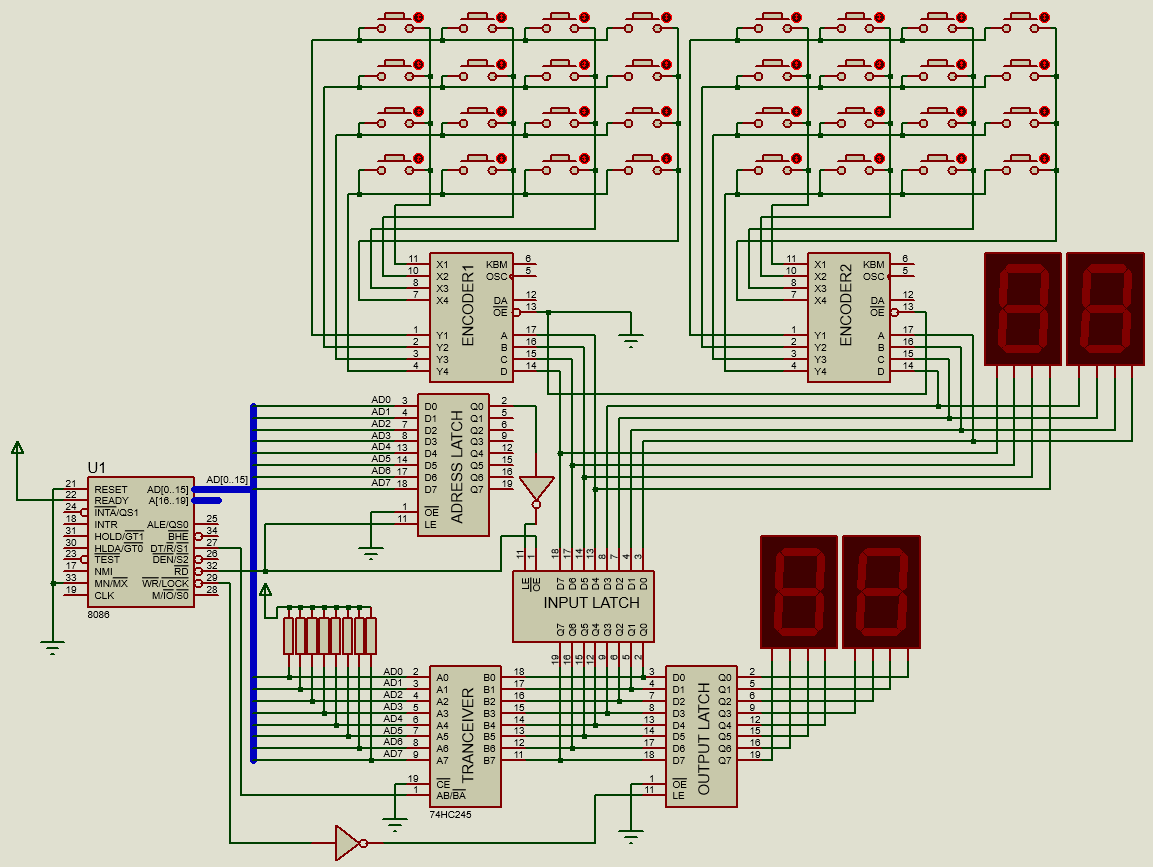
\includegraphics[width=21cm]{Tasarım2.png}
	\caption{Input/Output}
	\label{Tasarım}
\end{sidewaysfigure}
\begin{sidewaysfigure}[h!]
	\centering
	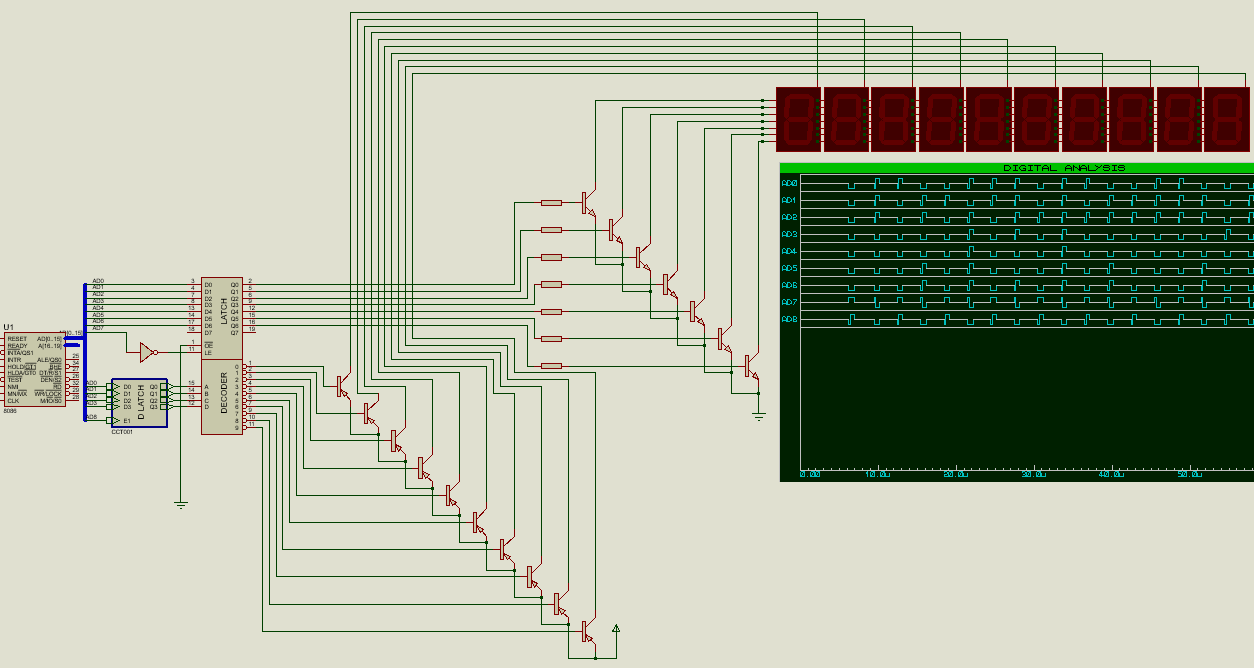
\includegraphics[width=21cm]{Tasarım.png}
	\caption{10 digit 7-segment display}
	\label{Tasarım2}
\end{sidewaysfigure}
\begin{sidewaysfigure}[h!]
	\centering
	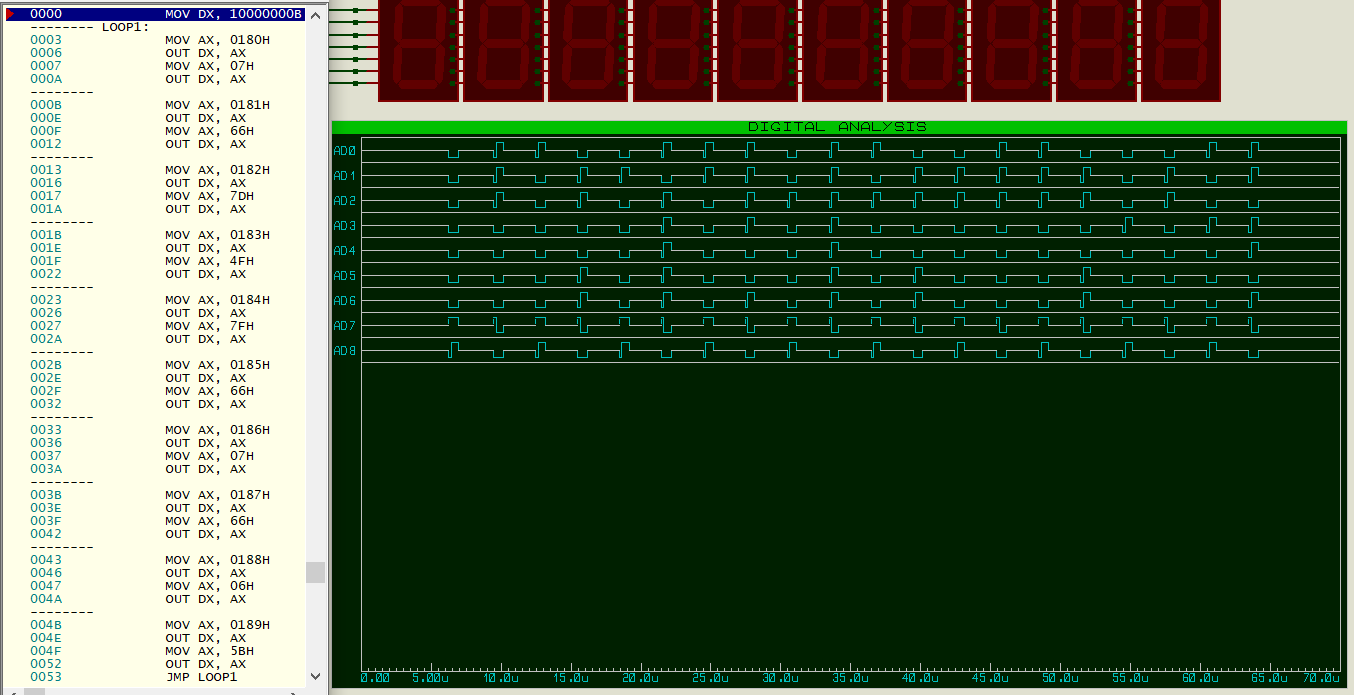
\includegraphics[width=21cm]{Graph.png}
	\caption{Logic analysis}
	\label{Analiz}
\end{sidewaysfigure}
\end{document}
